\documentclass[12pt, oneside]{book}
\usepackage[a4paper,top=2.5cm,bottom=2.5cm,left=3.5cm,right=2cm]{geometry}
\usepackage[utf8]{inputenc}
\usepackage[T1]{fontenc}
\usepackage{graphicx}
\usepackage{bibentry}
\usepackage{url}
\usepackage{mathtools}
\usepackage{textcomp}
\usepackage{listings}
\usepackage{python}
\usepackage[slovak]{babel} % vypnite pre prace v anglictine
\linespread{1.25} % hodnota 1.25 by mala zodpovedat 1.5 riadkovaniu


% Default fixed font does not support bold face

% Custom colors
\usepackage{color}
\definecolor{deepblue}{rgb}{0,0,0.5}
\definecolor{deepred}{rgb}{0.6,0,0}
\definecolor{deepgreen}{rgb}{0,0.5,0}

\definecolor{lightgray}{rgb}{.9,.9,.9}
\definecolor{darkgray}{rgb}{.4,.4,.4}
\definecolor{purple}{rgb}{0.65, 0.12, 0.82}



% -------------------
% --- Definicia zakladnych pojmov
% --- Vyplnte podla vasho zadania
% -------------------
\def\mfrok{2016}
\def\mfnazov{Interaktívny portál na vyučovanie dynamického programovania}
\def\mftyp{Bakalárska práca}
\def\mfautor{Michal Smolík}
\def\mfskolitel{Michal Foríšek, PhD }




%ak mate konzultanta, odkomentujte aj jeho meno na titulnom liste
%\def\mfkonzultant{tit. Meno Priezvisko, tit. }

\def\mfmiesto{Bratislava, \mfrok}



%aj cislo odboru je povinne a je podla studijneho odboru autora prace
\def\mfodbor{2508 Informatika}
\def\program{ Informatika }
\def\mfpracovisko{ Katedra informatiky }

\begin{document}

\nobibliography*
% -------------------
% --- Obalka ------
% -------------------
\thispagestyle{empty}

\begin{center}
\sc\large
Univerzita Komenského v Bratislave\\
Fakulta matematiky, fyziky a informatiky

\vfill

{\LARGE\mfnazov}\\
\mftyp
\end{center}

\vfill

{\sc\large
\noindent \mfrok\\
\mfautor
}

\eject % EOP i
% --- koniec obalky ----

% -------------------
% --- Titulný list
% -------------------

\thispagestyle{empty}
\noindent

\begin{center}
\sc
\large
Univerzita Komenského v Bratislave\\
Fakulta matematiky, fyziky a informatiky

\vfill

{\LARGE\mfnazov}\\
\mftyp
\end{center}

\vfill

\noindent
\begin{tabular}{ll}
Študijný program: & \program \\
Študijný odbor: & \mfodbor \\
Školiace pracovisko: & \mfpracovisko \\
Školiteľ: & \mfskolitel \\
% Konzultant: & \mfkonzultant \\
\end{tabular}

\vfill


\noindent \mfmiesto\\
\mfautor

\eject % EOP i


% --- Koniec titulnej strany


% -------------------
% --- Zadanie z AIS
% -------------------
% v tlačenej verzii s podpismi zainteresovaných osôb.
% v elektronickej verzii sa zverejňuje zadanie bez podpisov

\newpage
\thispagestyle{empty}
\centerline{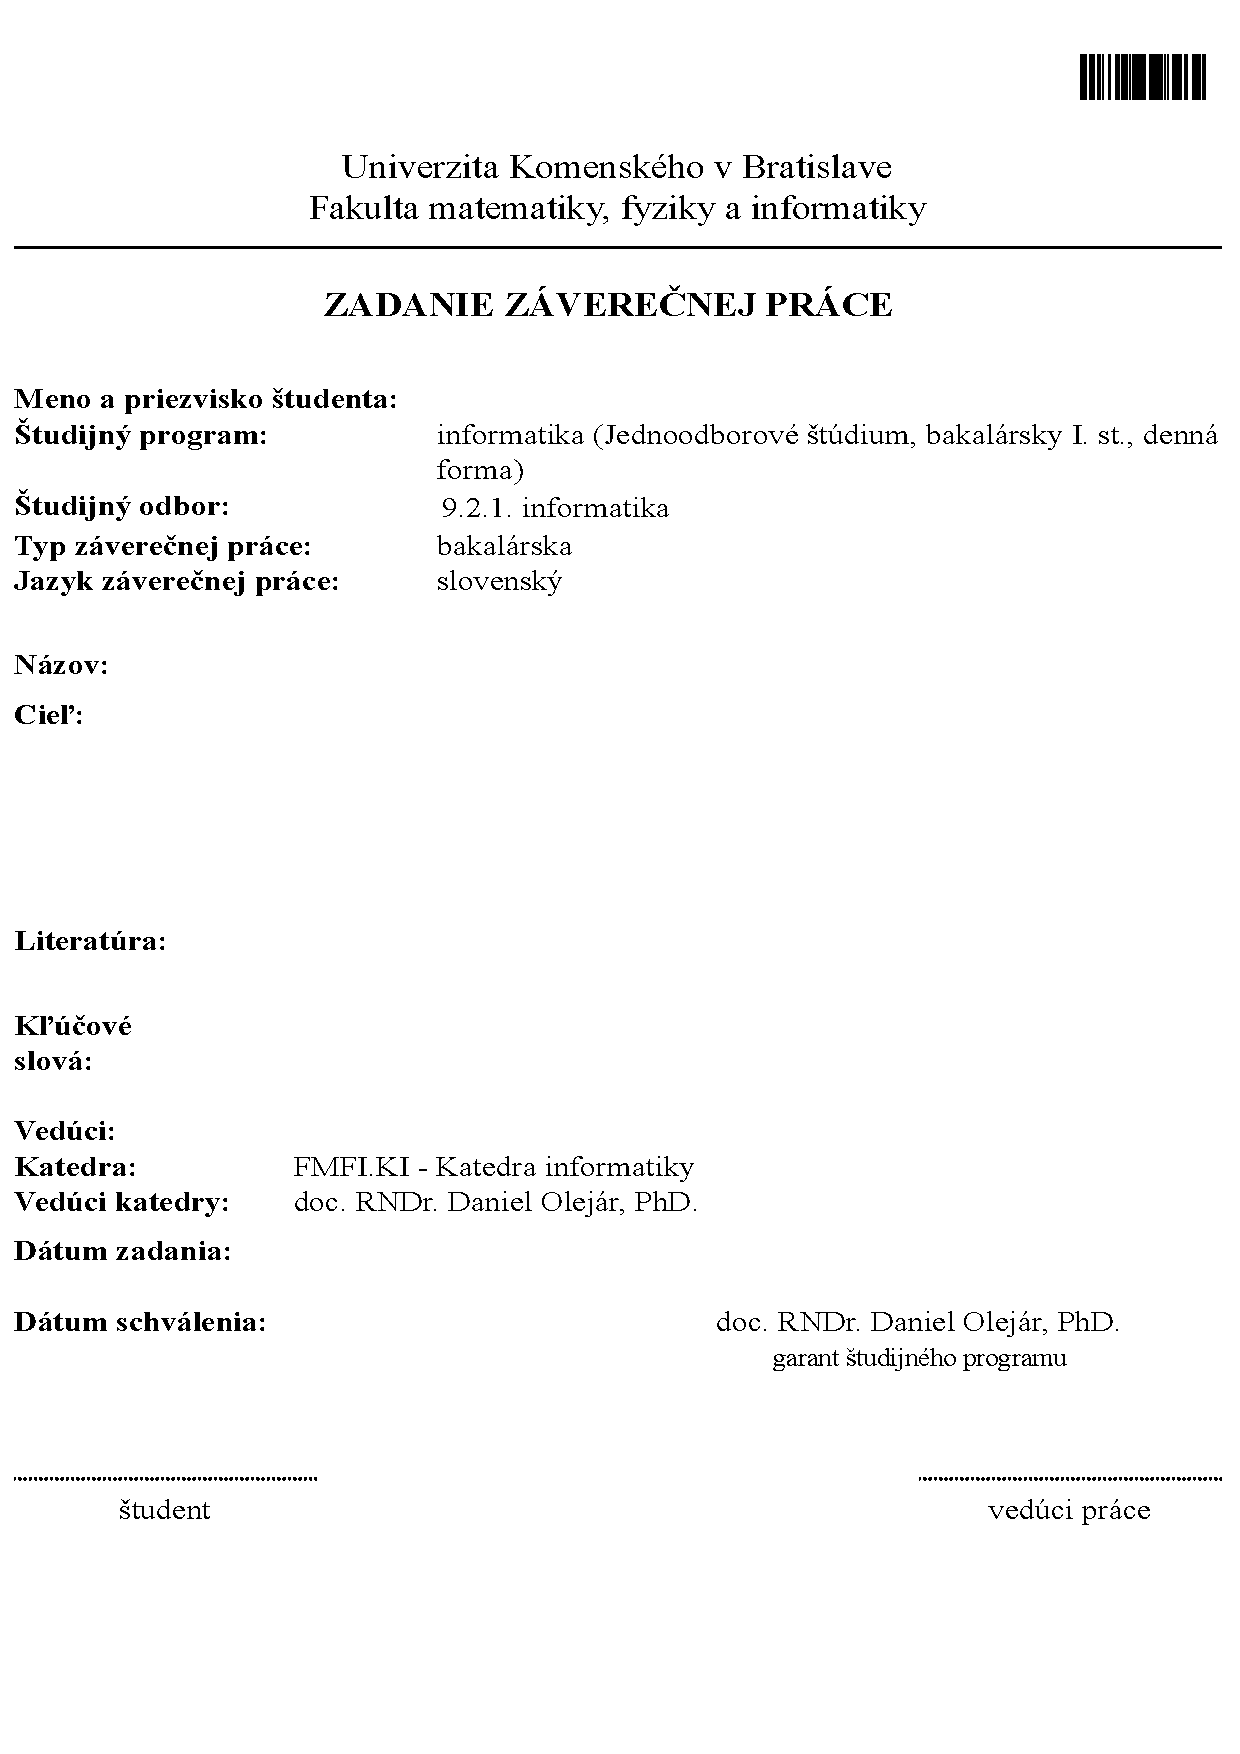
\includegraphics[width=\paperwidth]{images/zadanie}}

% --- Koniec zadania

\frontmatter

% -------------------
%   Poďakovanie - nepovinné
% -------------------
\setcounter{page}{3}
\newpage
~

\vfill
{\bf Poďakovanie:}

% --- Koniec poďakovania

% -------------------
%   Abstrakt - Slovensky
% -------------------
\newpage
\section*{Abstrakt}
Táto práca sa zaoberá implementáciou interaktívneho portálu na vyučovanie
dynamického programovania. Výučba na našom portáli prebieha hlavne riešením
implementačných úloh, ktoré automaticky testujeme. Portál má aj kapacitu
sledovať postup používateľov a náročnosť úloh. Práca obsahuje aj
interaktívnu vizualizáciu rekurzívnych a memoizovaných funkcií.

Portál pozostáva z Django databázového servera a jednoduchého HTML používateľského prostredia.

\paragraph*{Kľúčové slová:}Dynamické programovanie, Výučba porgramovania, Vizualizácia
% jedno, druhé, tretie (prípadne štvrté, piate)
% --- Koniec Abstrakt - Slovensky


% -------------------
% --- Abstrakt - Anglicky
% -------------------
\newpage
\section*{Abstract}
This thesis is about implementation of interactive portal for teaching
of dynamic programming. Learning process on our portal consists mainly of
implementation lessons, which are automatically tested. Portal also has capacity
to monitor users' progress and difficulty of lessons. Thesis also contains
an interactive visualisation of recursive and memoized functions.

\paragraph*{Keywords:} Dynamic programming, Teaching of programming, Visualisation

% --- Koniec Abstrakt - Anglicky

% -------------------
% --- Predhovor - v informatike sa zvacsa nepouziva
% -------------------
%\newpage
%\thispagestyle{empty}
%
%\huge{Predhovor}
%\normalsize
%\newline
%Predhovor je všeobecná informácia o práci, obsahuje hlavnú charakteristiku práce
%a okolnosti jej vzniku. Autor zdôvodní výber témy, stručne informuje o cieľoch
%a význame práce, spomenie domáci a zahraničný kontext, komu je práca určená,
%použité metódy, stav poznania; autor stručne charakterizuje svoj prístup a svoje
%hľadisko.
%
% --- Koniec Predhovor


% -------------------
% --- Obsah
% -------------------

\newpage

\tableofcontents

% ---  Koniec Obsahu

% -------------------
% --- Zoznamy tabuliek, obrázkov - nepovinne
% -------------------

%\newpage

%\listoffigures

% ---  Koniec Zoznamov

\mainmatter


\input uvod.tex

\input specifikacie.tex

\input front-end.tex

%\input features.tex

\input server.tex

\input front-end-impl.tex

\input dokumentacia.tex



\input future.tex

%\input lorem.tex

\input zaver.tex

% -------------------
% --- Bibliografia
% -------------------


\newpage

\backmatter

\thispagestyle{empty}
\nocite{*}
\clearpage


\bibliographystyle{plain}
\bibliography{literatura}

%Prípadne môžete napísať literatúru priamo tu
\begin{thebibliography}{1}

\bibitem{Django}
Django documentation.
\newblock \url{https://docs.djangoproject.com/en/1.9/}.
\newblock [2016-5-10].

\bibitem{FBlogin}
Facebook login for the web with the javascript sdk.
\newblock \url{https://developers.facebook.com/docs/facebook-login/web}.
\newblock [2015-12-07].

\bibitem{rest}
Rest framework documentation.
\newblock \url{http://www.django-rest-framework.org/}.
\newblock [2016-5-10].

\bibitem{visualgo}
VisuAlgo.
\newblock \url{http://visualgo.net/recursion}.
\newblock [2016-5-11].

\bibitem{misof}
Michal Foríšek.
\newblock Security of programming contest systems.
\newblock {\em Information Technologies at School 2006, pp. 553--563.}

\bibitem{mares}
Bernard~Blackham Martin~Mareš.
\newblock A new contest sandbox.
\newblock {\em Olympiads in informatics, 2012, Vol. 6, 100-109}

\end{thebibliography}

%---koniec Referencii

% -------------------
%--- Prilohy---
% -------------------

%Nepovinná časť prílohy obsahuje materiály, ktoré neboli zaradené priamo  do textu. Každá príloha sa začína na novej strane.
%Zoznam príloh je súčasťou obsahu.
%
%\addcontentsline{toc}{chapter}{Appendix A}
%\input AppendixA.tex
%
%\addcontentsline{toc}{chapter}{Appendix B}
%\input AppendixB.tex

\end{document}
